\documentclass{standalone}
\usepackage{tikz}
\usetikzlibrary{patterns, positioning}

\begin{document}
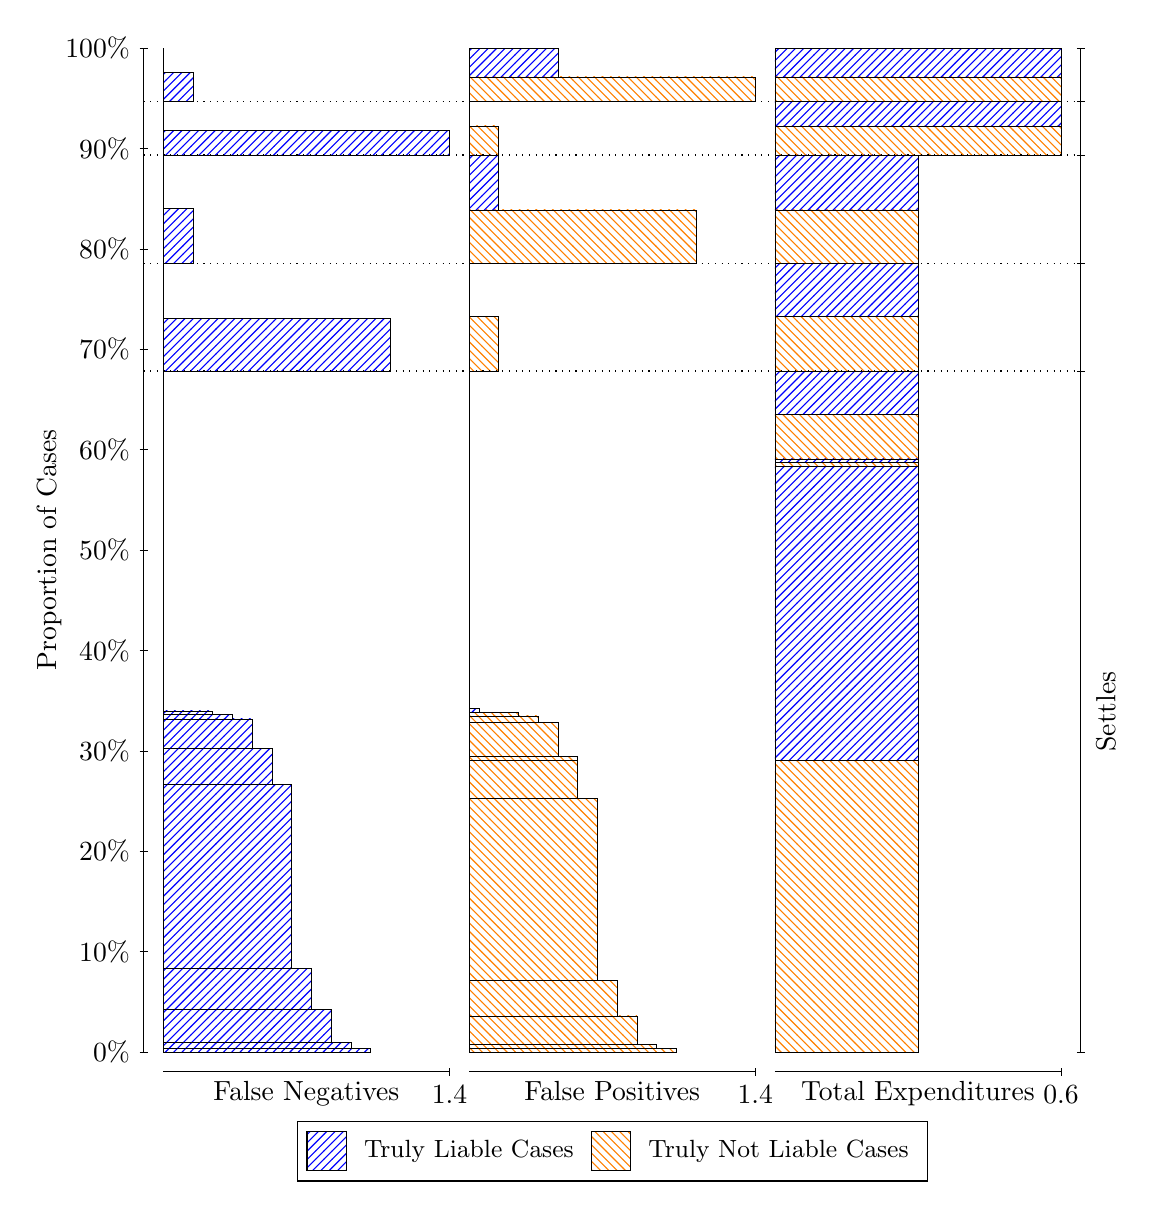
\begin{tikzpicture}
\draw[black, very thin] (1.5,1.75) -- (1.5,14.5);
\node[rotate=90, anchor=center] at (0.3, 8.125) {Proportion of Cases};
\draw[black, very thin] (1.45,1.75) -- (1.55,1.75);
\node[anchor=east] at (1.45, 1.75) {0\%};
\draw[black, very thin] (1.45,3.025) -- (1.55,3.025);
\node[anchor=east] at (1.45, 3.025) {10\%};
\draw[black, very thin] (1.45,4.3) -- (1.55,4.3);
\node[anchor=east] at (1.45, 4.3) {20\%};
\draw[black, very thin] (1.45,5.575) -- (1.55,5.575);
\node[anchor=east] at (1.45, 5.575) {30\%};
\draw[black, very thin] (1.45,6.85) -- (1.55,6.85);
\node[anchor=east] at (1.45, 6.85) {40\%};
\draw[black, very thin] (1.45,8.125) -- (1.55,8.125);
\node[anchor=east] at (1.45, 8.125) {50\%};
\draw[black, very thin] (1.45,9.4) -- (1.55,9.4);
\node[anchor=east] at (1.45, 9.4) {60\%};
\draw[black, very thin] (1.45,10.675) -- (1.55,10.675);
\node[anchor=east] at (1.45, 10.675) {70\%};
\draw[black, very thin] (1.45,11.95) -- (1.55,11.95);
\node[anchor=east] at (1.45, 11.95) {80\%};
\draw[black, very thin] (1.45,13.225) -- (1.55,13.225);
\node[anchor=east] at (1.45, 13.225) {90\%};
\draw[black, very thin] (1.45,14.5) -- (1.55,14.5);
\node[anchor=east] at (1.45, 14.5) {100\%};

\draw[black, very thin] (13.4,1.75) -- (13.4,14.5);
\draw[black, very thin] (13.35,1.75) -- (13.45,1.75);
\node[anchor=west] at (13.35, 1.75) {};
\draw[black, very thin] (13.35,10.398) -- (13.45,10.398);
\node[anchor=west] at (13.35, 10.398) {};
\draw[black, very thin] (13.35,11.763) -- (13.45,11.763);
\node[anchor=west] at (13.35, 11.763) {};
\draw[black, very thin] (13.35,13.142) -- (13.45,13.142);
\node[anchor=west] at (13.35, 13.142) {};
\draw[black, very thin] (13.35,13.822) -- (13.45,13.822);
\node[anchor=west] at (13.35, 13.822) {};
\draw[black, very thin] (13.35,14.5) -- (13.45,14.5);
\node[anchor=west] at (13.35, 14.5) {};

\draw[black, very thin, pattern color=blue, pattern=north east lines] (1.75,1.75) rectangle (4.381,1.7961);
\draw[black, very thin, pattern color=blue, pattern=north east lines] (1.75,1.7961) rectangle (4.1305,1.8715);
\draw[black, very thin, pattern color=blue, pattern=north east lines] (1.75,1.8715) rectangle (3.8799,2.2893);
\draw[black, very thin, pattern color=blue, pattern=north east lines] (1.75,2.2893) rectangle (3.6293,2.8153);
\draw[black, very thin, pattern color=blue, pattern=north east lines] (1.75,2.8153) rectangle (3.3787,5.1447);
\draw[black, very thin, pattern color=blue, pattern=north east lines] (1.75,5.1447) rectangle (3.1282,5.6075);
\draw[black, very thin, pattern color=blue, pattern=north east lines] (1.75,5.6075) rectangle (2.8776,5.9814);
\draw[black, very thin, pattern color=blue, pattern=north east lines] (1.75,5.9814) rectangle (2.627,6.0342);
\draw[black, very thin, pattern color=blue, pattern=north east lines] (1.75,6.0342) rectangle (2.3764,6.0811);
\draw[black, very thin, pattern color=orange, pattern=north west lines] (1.75,6.0811) rectangle (1.75,10.398);
\draw[black, very thin, pattern color=blue, pattern=north east lines] (1.75,10.398) rectangle (4.6316,11.067);
\draw[black, very thin, pattern color=orange, pattern=north west lines] (1.75,11.067) rectangle (1.75,11.763);
\draw[black, very thin, pattern color=blue, pattern=north east lines] (1.75,11.763) rectangle (2.1259,12.46);
\draw[black, very thin, pattern color=orange, pattern=north west lines] (1.75,12.46) rectangle (1.75,13.142);
\draw[black, very thin, pattern color=blue, pattern=north east lines] (1.75,13.142) rectangle (5.3833,13.453);
\draw[black, very thin, pattern color=orange, pattern=north west lines] (1.75,13.453) rectangle (1.75,13.822);
\draw[black, very thin, pattern color=blue, pattern=north east lines] (1.75,13.822) rectangle (2.1259,14.187);
\draw[black, very thin, pattern color=orange, pattern=north west lines] (1.75,14.187) rectangle (1.75,14.5);
\draw[black, very thin, pattern color=orange, pattern=north west lines] (5.6333,1.75) rectangle (8.2644,1.7957);
\draw[black, very thin, pattern color=orange, pattern=north west lines] (5.6333,1.7957) rectangle (8.0138,1.8482);
\draw[black, very thin, pattern color=orange, pattern=north west lines] (5.6333,1.8482) rectangle (7.7632,2.2096);
\draw[black, very thin, pattern color=orange, pattern=north west lines] (5.6333,2.2096) rectangle (7.5126,2.6584);
\draw[black, very thin, pattern color=orange, pattern=north west lines] (5.6333,2.6584) rectangle (7.2621,4.9677);
\draw[black, very thin, pattern color=orange, pattern=north west lines] (5.6333,4.9677) rectangle (7.0115,5.4502);
\draw[black, very thin, pattern color=orange, pattern=north west lines] (5.6333,5.4502) rectangle (7.0115,5.505);
\draw[black, very thin, pattern color=orange, pattern=north west lines] (5.6333,5.505) rectangle (6.7609,5.9394);
\draw[black, very thin, pattern color=orange, pattern=north west lines] (5.6333,5.9394) rectangle (6.5103,6.0187);
\draw[black, very thin, pattern color=orange, pattern=north west lines] (5.6333,6.0187) rectangle (6.2598,6.0666);
\draw[black, very thin, pattern color=blue, pattern=north east lines] (5.6333,6.0666) rectangle (5.7586,6.1135);
\draw[black, very thin, pattern color=blue, pattern=north east lines] (5.6333,6.1135) rectangle (5.6333,10.398);
\draw[black, very thin, pattern color=orange, pattern=north west lines] (5.6333,10.398) rectangle (6.0092,11.093);
\draw[black, very thin, pattern color=blue, pattern=north east lines] (5.6333,11.093) rectangle (5.6333,11.763);
\draw[black, very thin, pattern color=orange, pattern=north west lines] (5.6333,11.763) rectangle (8.5149,12.445);
\draw[black, very thin, pattern color=blue, pattern=north east lines] (5.6333,12.445) rectangle (6.0092,13.142);
\draw[black, very thin, pattern color=orange, pattern=north west lines] (5.6333,13.142) rectangle (6.0092,13.511);
\draw[black, very thin, pattern color=blue, pattern=north east lines] (5.6333,13.511) rectangle (5.6333,13.822);
\draw[black, very thin, pattern color=orange, pattern=north west lines] (5.6333,13.822) rectangle (9.2667,14.134);
\draw[black, very thin, pattern color=blue, pattern=north east lines] (5.6333,14.134) rectangle (6.7609,14.5);
\draw[black, very thin, pattern color=orange, pattern=north west lines] (9.5167,1.75) rectangle (11.333,5.4502);
\draw[black, very thin, pattern color=blue, pattern=north east lines] (9.5167,5.4502) rectangle (11.333,9.1882);
\draw[black, very thin, pattern color=orange, pattern=north west lines] (9.5167,9.1882) rectangle (11.333,9.2361);
\draw[black, very thin, pattern color=blue, pattern=north east lines] (9.5167,9.2361) rectangle (11.333,9.2822);
\draw[black, very thin, pattern color=orange, pattern=north west lines] (9.5167,9.2822) rectangle (11.333,9.8507);
\draw[black, very thin, pattern color=blue, pattern=north east lines] (9.5167,9.8507) rectangle (11.333,10.398);
\draw[black, very thin, pattern color=orange, pattern=north west lines] (9.5167,10.398) rectangle (11.333,11.093);
\draw[black, very thin, pattern color=blue, pattern=north east lines] (9.5167,11.093) rectangle (11.333,11.763);
\draw[black, very thin, pattern color=orange, pattern=north west lines] (9.5167,11.763) rectangle (11.333,12.445);
\draw[black, very thin, pattern color=blue, pattern=north east lines] (9.5167,12.445) rectangle (11.333,13.142);
\draw[black, very thin, pattern color=orange, pattern=north west lines] (9.5167,13.142) rectangle (13.15,13.511);
\draw[black, very thin, pattern color=blue, pattern=north east lines] (9.5167,13.511) rectangle (13.15,13.822);
\draw[black, very thin, pattern color=orange, pattern=north west lines] (9.5167,13.822) rectangle (13.15,14.134);
\draw[black, very thin, pattern color=blue, pattern=north east lines] (9.5167,14.134) rectangle (13.15,14.5);
\draw[black, dotted] (1.5,10.398) -- (13.4,10.398);
\draw[black, dotted] (1.5,11.763) -- (13.4,11.763);
\draw[black, dotted] (1.5,13.142) -- (13.4,13.142);
\draw[black, dotted] (1.5,13.822) -- (13.4,13.822);
\draw[black, very thin] (1.75,1.5) -- (5.3833,1.5);
\node[anchor=north] at (3.5667, 1.5) {False Negatives};
\draw[black, very thin] (5.3833,1.45) -- (5.3833,1.55);
\node[anchor=north] at (5.3833, 1.45) {1.4};

\draw[black, very thin] (5.6333,1.5) -- (9.2667,1.5);
\node[anchor=north] at (7.45, 1.5) {False Positives};
\draw[black, very thin] (9.2667,1.45) -- (9.2667,1.55);
\node[anchor=north] at (9.2667, 1.45) {1.4};

\draw[black, very thin] (9.5167,1.5) -- (13.15,1.5);
\node[anchor=north] at (11.333, 1.5) {Total Expenditures};
\draw[black, very thin] (13.15,1.45) -- (13.15,1.55);
\node[anchor=north] at (13.15, 1.45) {0.6};

\node[black, centered, rotate=90] at (13.72, 6.0739) {Settles};





\draw (7.449999999999999,1.5) node[draw=none] (baseCoordinate) {};
\begin{scope}[align=center]
        \matrix[scale=0.5, draw=black, below=0.5cm of baseCoordinate, nodes={draw}, column sep=0.1cm]{
            \node[rectangle, draw, minimum width=0.5cm, minimum height=0.5cm, pattern=north east lines, pattern color=blue] {}; &
            \node[draw=none, font=\small] (B) {Truly Liable Cases}; &
            \node[rectangle, draw, minimum width=0.5cm, minimum height=0.5cm, pattern=north west lines, pattern color=orange] {}; &
            \node[draw=none, font=\small] (B) {Truly Not Liable Cases}; \\
            };
\end{scope}

\end{tikzpicture}
\end{document}